\vspace{0.015\textheight}
Physics has been the ultimate driving force behind all of the technological advances mankind has accomplished. There have always been unanswered questions that force physicists to search for answers. One example of these questions has to do with \newterm{mass}: what is mass, and via what mechanism is it generated? In order to answer these questions, one needs to understand the fundamental constituents of the universe and their interactions.

The nature of matter began as a philosophical concept in ancient Greece. Elementary particle physics has roots dating back to 450 BC when Empedocles imagined the fundamental elements to be fire, earth, air, and water. The forces of attraction and repulsion allowed these elements to interact. Modern particle physics started to evolve in the early 19\textsuperscript{th} century with the discovery of pure chemical elements, and this led to the resurgence of the concept of the \newterm{atom}. The concept of the atom was first proposed by early Greeks and Indian philosophers as the smallest indivisible particle. In the late 19\textsuperscript{th} and early 20\textsuperscript{th} centuries, the discoveries of radioactivity by Henri Becquerel and the nucleus in Rutherford's famous gold foil experiment showed that actual atoms have substructure and are more complex than initially anticipated. Experimental evidence suggested that the atom is made out of simpler particles: electrons ($e^{-}$), protons ($p^{+}$), and neutrons ($n^{0}$), where protons and neutrons form the nucleus and the electrons hover around it.

Over time, more questions started to arise like ``What is the mechanism of radioactivity?''  and ``How do positively charged protons stay so closely packed inside the nucleus?''  In 1932, Carl Anderson discovered the first \newterm{antiparticle} of the electron, the positron ($e^{+}$), proposed by Paul Dirac in 1927. Several years later, while studying cosmic rays, a much heavier version of the electron, the muon ($\mu$), was discovered by Anderson together with Seth Neddermeyer. These discoveries, which were so incongruous and surprising at that time, laid the foundation for a new category of fundamental particles called \newterm{leptons}.

In the middle of the 20\textsuperscript{th} century, another flurry of tiny particles called \newterm{hadrons} were discovered in experimental laboratories. These particles were explained by Murray Gell-Mann and Kazuhiko Nishijima by the introduction of a new set of fundamental particles called \newterm{quarks}. Their quark model suggested that quarks have fractional charges and that there are many types of quarks with different electric charges and different quantum numbers. The quark model was able to categorize and explain this ``zoo'' of hadrons, but was not able to explain the more fundamental questions such as what gives particles their mass.

The present theory of particle physics is known as the Standard Model (SM). At the heart of the SM are the matter particles: six quarks and six leptons. For each of these particles there is an antiparticle with an identical mass but with opposite quantum numbers such as electric charge. The quarks and leptons make up all the visible matter. In addition, there are four force-mediating particles that govern the interactions of the aforementioned particles and antiparticles (see Fig.~\ref{fig_SMparticlesComplete}).

\begin{figure}[htb!]
\centering
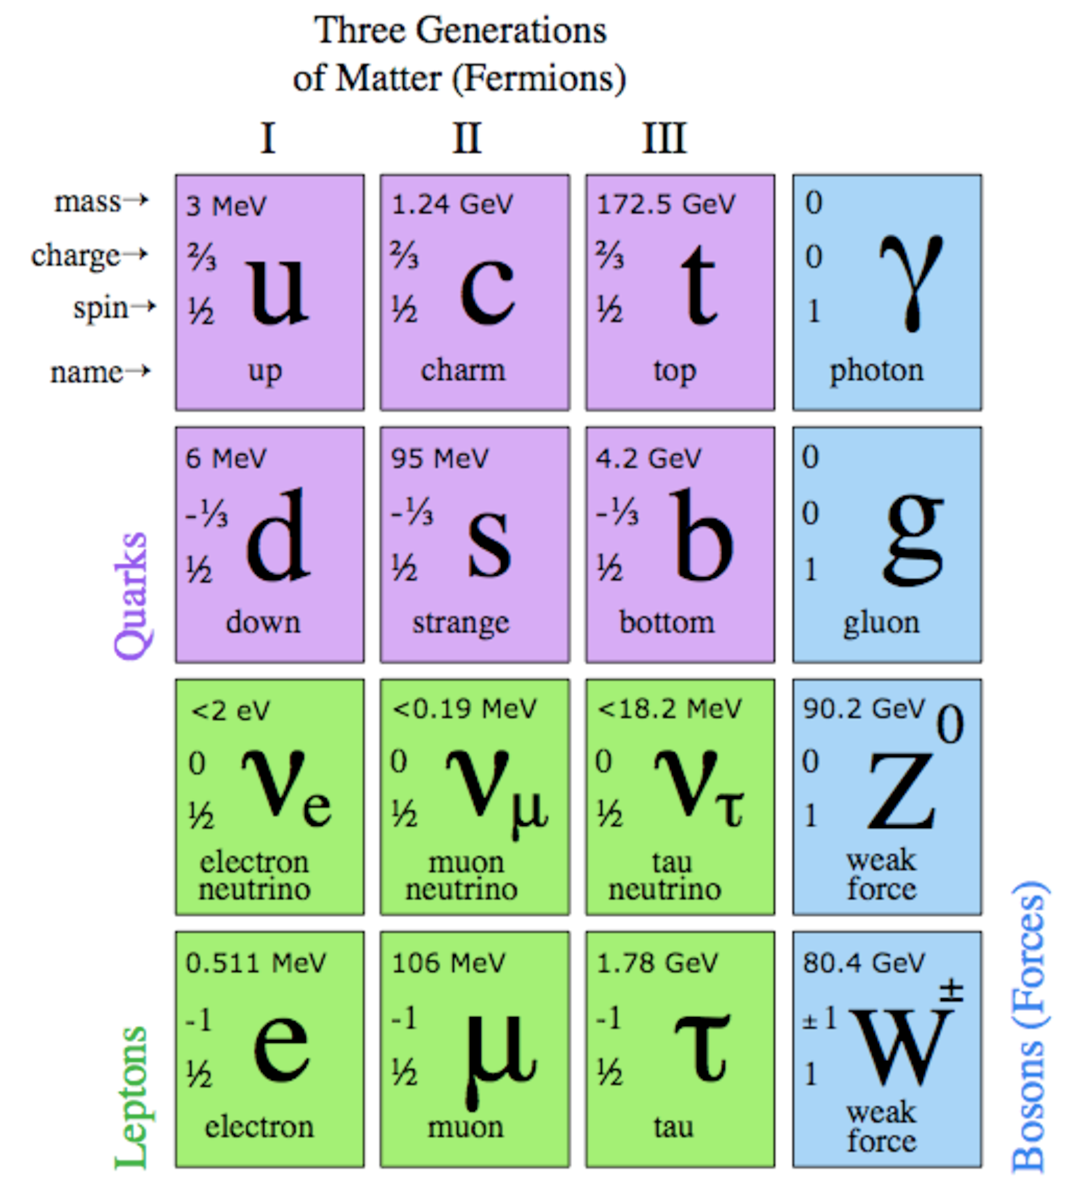
\includegraphics[scale=0.5]{SM_particlesComplete.pdf}
\caption[Summary of Standard Model particles and forces.]{The building blocks of the Standard Model: six types of quarks, six types of leptons, and four force-mediating bosons. Each quark and lepton has an antiparticle with identical mass but opposite electric charge. The final piece of the puzzle, the Higgs particle, has yet to be seen.
\label{fig_SMparticlesComplete}}
\end{figure}

The quarks are arranged in three generations. The 2\textsuperscript{nd} and 3\textsuperscript{rd} generations are heavier copies of the 1\textsuperscript{st} generation. The same is true with the leptons.

\vspace{-0.015\textheight}
\begin{singlespace}
\begin{itemize}
\item {1\textsuperscript{st} generation --- The up quark ($u$) and down quark ($d$) form the first generation. Almost all visible and stable matter is composed of these two light quarks. Their antiparticles are the $\bar{u}$ ($u$-bar) and $\bar{d}$ ($d$-bar).}
\item {2\textsuperscript{nd} generation --- The charmed quark ($c$) and strange ($s$) quark and their antiparticles, $\bar{c}$ and $\bar{s}$, form the 2\textsuperscript{nd} generation.}
\item {3\textsuperscript{rd} generation --- The top ($t$) and bottom ($b$) quarks and their antiparticles, $\bar{t}$ and $\bar{b}$, form the 3\textsuperscript{rd} generation. The top quark is the heaviest of all quarks with a mass of 173.3~$\pm$~1.1~\massunits according to the latest measurements~\cite{pap:TopMass}.}
\end{itemize}
 \end{singlespace}

The six types of quarks are called \newterm{flavors}. Each flavor of quark has one of three values of \newterm{color} charge. The color charge can be red, blue, and green for particles, and antired, antiblue, and antigreen for antiparticles.

There are six leptons: three charged and three neutral (see Fig.~\ref{fig_SMparticlesComplete}). The leptons are assumed to be point-like particles and so far there is no evidence of any internal structure. The muon ($\mu^{-}$) and tau ($\tau^{-}$) are heavier replicas of the lightest lepton, the electron ($e^{-}$). Electrons are the most abundant of the three and are found in ordinary matter. There are three corresponding neutrinos ($\nu$): the electron neutrino ($\nu_{e}$), muon neutrino ($\nu_{\mu}$), and tau neutrino ($\nu_{\tau}$). Neutrinos are assumed to be massless point-like particles in the SM. However, recent experimental evidence suggests they may have tiny mass \cite{pap:PDG}. The SM assumes quarks and leptons to be spin-1/2 particles. Particles with half-integer spin are termed \newterm{fermions}, which follow Fermi--Dirac statistics. Fermions obey the Pauli Exclusion Principle, which states that no two identical fermions may occupy the same quantum state simultaneously. Particles with integer spin are termed \newterm{bosons} and follow Bose--Einstein statistics. Bosons, unlike fermions, are not required to obey the Pauli Exclusion Principle. As mentioned earlier, hadrons are formed by combining quarks and antiquarks. In forming such combinations, one has to conserve quantum numbers such as baryon number, lepton number, color charge, and electric charge.

%%%%%%%%%%%%%%%%%%%%%%%%%
Interactions among fundamental particles can be classified in many ways. Historically this was done on the basis of their strengths. This leads to four types of interactions: \newterm{strong}, \newterm{electromagnetic}, \newterm{weak}, and \newterm{gravitational}.

The Standard Model has proposed four force-mediating particles. The photon ($\gamma$), a massless particle with no electric charge, mediates electromagnetic interactions as described by Quantum Electrodynamics (QED). The \newterm{gluon} is a massless particle that engages in strong interactions between color-carrying particles. Lastly, the \W and \Z bosons are believed to facilitate the weak interactions.  These are massive particles that can change the flavor of quarks and thereby the quark composition of particles.  Figure~\ref{fig:SMinteractions} illustrates these interactions. Finally, the gravitational force is assumed to be mediated by the \newterm{graviton}, but the SM does not account for gravity in its formulation, as it is very weak. The details of these interactions will be discussed in the next chapter. Table~\ref{tab:summary_of_four_forces} summarizes these forces and their behavior.

\begin{figure}[htb!]
\centering
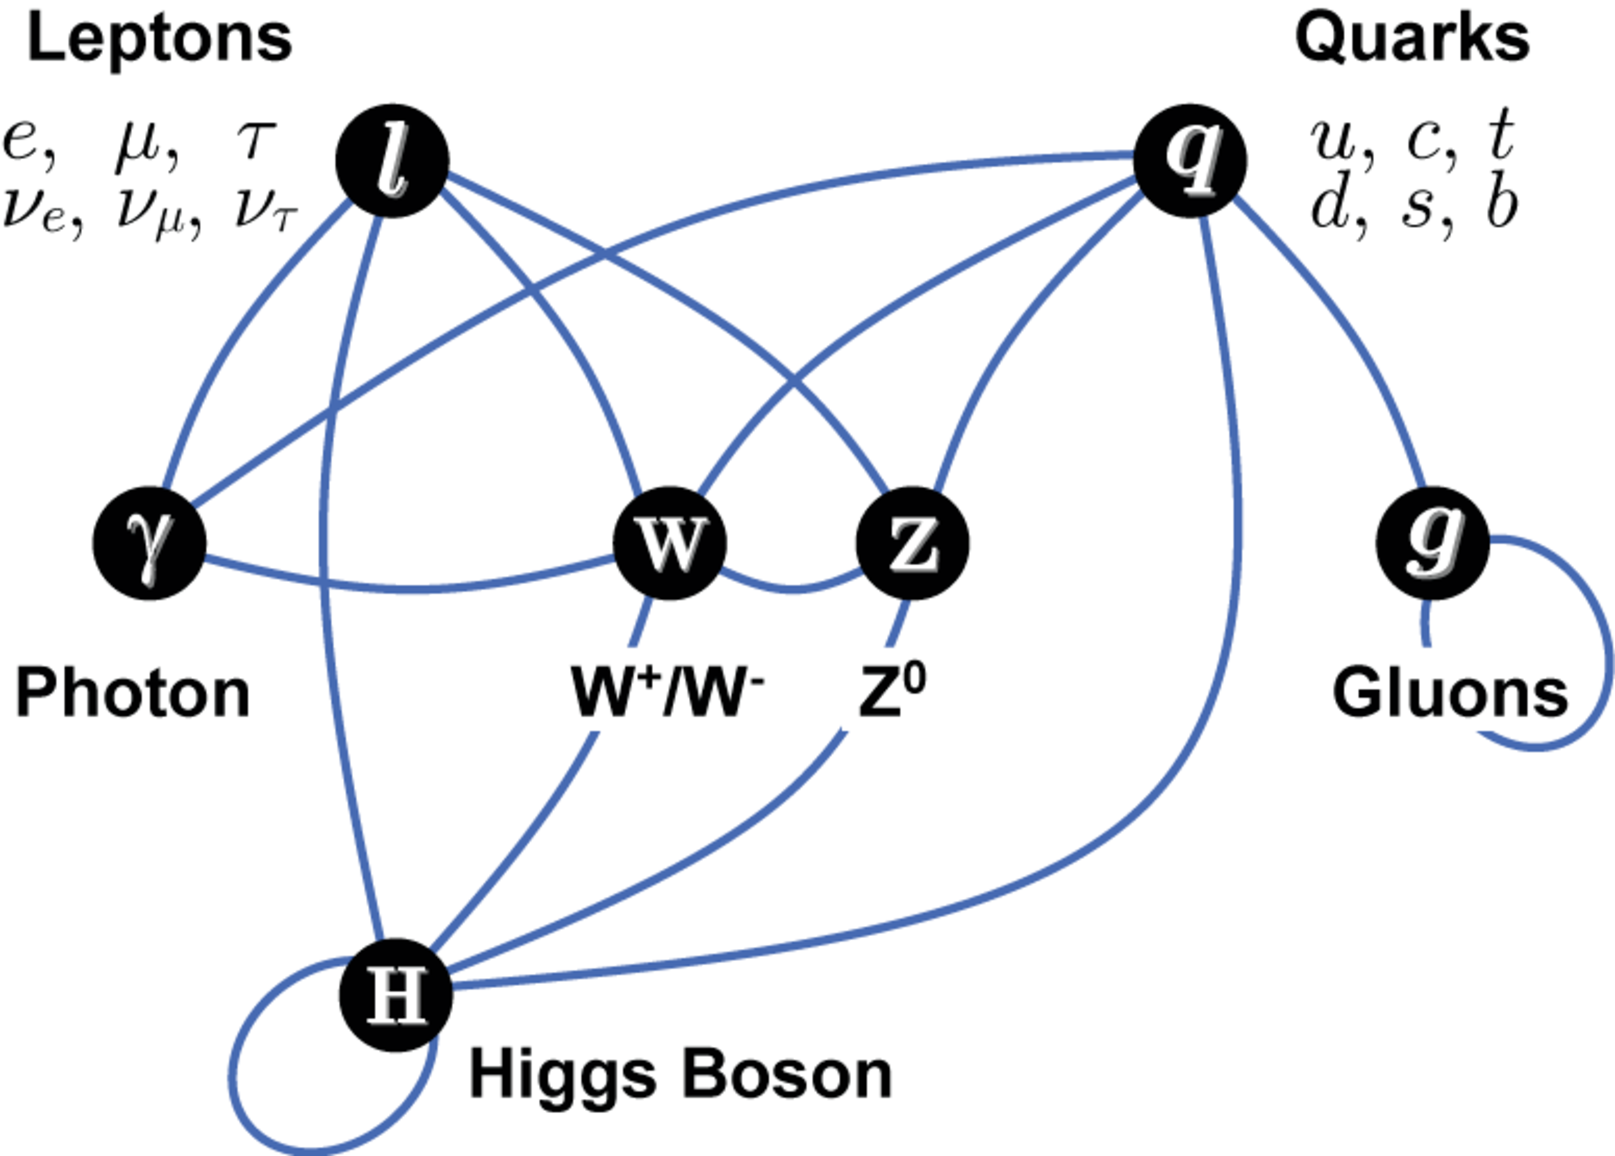
\includegraphics[scale=0.35]{Interactions.pdf}
\caption[Standard Model particles and force interactions.]{Diagram illustrating the possible interactions between elementary particles in the Standard Model. Vertices (darkened circles) represent types of particles, and the blue arcs connecting them represent possible interactions. The top row of vertices (leptons and quarks) are the matter particles; the second row of vertices (photon, $W$, $Z$, and gluon) are the force-mediating particles; the bottom row is the Higgs boson \cite{img_Interactions}.
\label{fig:SMinteractions}}
\end{figure}

\begin{table}[fhbt!]
\caption{Summary of the four fundamental forces with their relative strengths and range. The relative strength is given with respect to the strength of the graviton. This table should only be used to understand the concepts involved, as the exact numbers are under constant scrutiny.}
\label{tab:summary_of_four_forces}
\centering
\begin{tabular}{lccccc}
\hline
\BUbf{Interaction} & \BUbf{Strong} & \BUbf{Electromagnetic} & \BUbf{Weak} & \BUbf{Gravitation}\\
\hline
\multirow{2}{*}{\BUbf{Theory}} & \multirow{2}{*}{QCD} & \multirow{2}{*}{QED} & Electroweak & General \\
& & & Theory & Relativity \\[1ex]
\BUbf{Mediators} & gluon ($g$) & photon ($\gamma$) & \W and \Z bosons & graviton \\[1ex]
\BUbf{Relative} & \multirow{2}{*}{$10^{38}$} & \multirow{2}{*}{$10^{36}$} & \multirow{2}{*}{$10^{25}$} & \multirow{2}{*}{1} \\
\BUbf{Strength} & & & &\\[1ex]
\BUbf{Long Distance} & \multirow{2}{*}{1} & \multirow{2}{*}{$\frac{1}{r^2}$} & \multirow{2}{*}{$\frac{1}{r} e^{-m_{W,Z} r}$} & \multirow{2}{*}{$\frac{1}{r^{2}}$} \\
\BUbf{Behavior} & & & & \\[1ex]
\BUbf{Range} & $10^{-15}$ & $\infty$ & $10^{-18}$ & $\infty$ \\
\hline
\end{tabular}
\end{table}

The electromagnetic and gravitational interactions have been known for a long time, as they are a part of our daily life in the macroscopic world. This is because they are long range interactions (compared to the size of the nucleus, which is $\sim$10$^{-12}$~cm). This long range behavior was explained by the introduction of the concept of a field, which is assumed to have an independent existence and most importantly, contains energy. It was James Maxwell in 1864 who took this idea and explained light as a propagating electromagnetic field. With the development of quantum mechanics, the field concept became more profound and explicit. In quantum mechanics, particles may have a dual particle-like and wave-like behavior as explained by Schr\"{o}dinger in 1926. Furthermore, this wave-like behavior implied that a particle's behavior cannot be predicted definitely; one can only determine probabilities of possible outcomes.

A charged object is assumed to constantly emit and absorb photons. For example, an electron passing by a proton might intercept such a photon, absorbing its momentum and thus changing course. The existence of these photons about a charged particle is possible due to Heisenberg's uncertainty principle, which says that position and momenta cannot be simultaneously measured to arbitrarily high precision. This led to the energy-time uncertainty $\Delta E \Delta t\gtrsim h$, where $h=4.1\times10^{-15}$~eV$\cdot$s is the Planck constant, which allows particles to exist for extremely short times without being required to abide by the law of conservation of energy. They are known as \newterm{virtual particles}. Essentially, virtual particles are an artifact of quantum field theory (QFT), in which the interactions between real particles are formulated by the exchange of virtual particles.

The Standard Model has no clear answers to some of the questions like why there are two extra families of leptons and quarks or why there are only three families altogether, why gravity is so weak, and why there is no prediction of the masses of quarks and leptons. Hence, a further understanding of these fundamental particles and their interactions is needed. But this is no easy task, as these particles do not exist in normal circumstances. In order to study them, they need to be produced artificially. In 1905, Einstein pointed out the mass-energy equivalence, $E=mc^{2}$, where $E$ is the energy, $m$ is the mass, and $c$ is the speed of light in a vacuum. This relationship implies that in order to create a particle at rest with a mass $m$, one needs an equivalent amount of energy given by $E=mc^{2}$. This brought the era of collider experiments. In collider experiments, two beams of particles are collided at high energies to produce these fundamental particles for closer observation. These collisions are studied using state-of-the-art detectors like the Collider Detector at Fermilab (CDF).

In order to answer some of the questions mentioned so far, an emerging technique known as a signature-based search is used to find new physics beyond what is predicted by the SM. This thesis is arranged as described below.

In the next chapter, the SM is further discussed to provide an overview of the present understanding of particle physics. It also explains the shortcomings of the SM. Then, a competing theory that extends the \SMtext, \GMSBtext (GSMB), is explained. This chapter also describe the underlying concepts of signature-based searches. Furthermore, it explains the photon + jets signature in both the SM and GSMB.

In Chapter 3, the experimental apparatus, the CDF detector, is explained in detail. The ``Monte Carlo Event Simulation'' chapter (Chapter 4) describes how a hard collision between two hadrons is understood and how such collisions are simulated. Chapter 5, titled ``Object Reconstruction and Identification,'' explains how final-state particles or ``objects'' such as electrons, positrons, photons, and jets are reconstructed in the detector. It also describes how additional physics quantities like missing transverse energy are derived from the reconstructed particles. In the ``Datasets and Event Selection'' chapter (Chapter 6), the data used in this analysis, including when and how they were collected, are described. Furthermore, it explains the selection criteria of photon + jets events for this analysis. The ``Background Modeling'' chapter (Chapter 7) explains processes in which a photon and jets are produced. The processes that produce real photons and fake photons in association with jets are elaborated upon. It also explains two methods of background modeling. The following chapter (Chapter~8) lists and explains possible systematic uncertainties and how they are quantified.

In the ``Results'' chapter (Chapter 9), the findings of this analysis and the implications of the results are discussed in detail. All measured physics quantities are shown with associated systematic uncertainties. In the last chapter (Chapter~10), the conclusion of this search for new physics is presented.